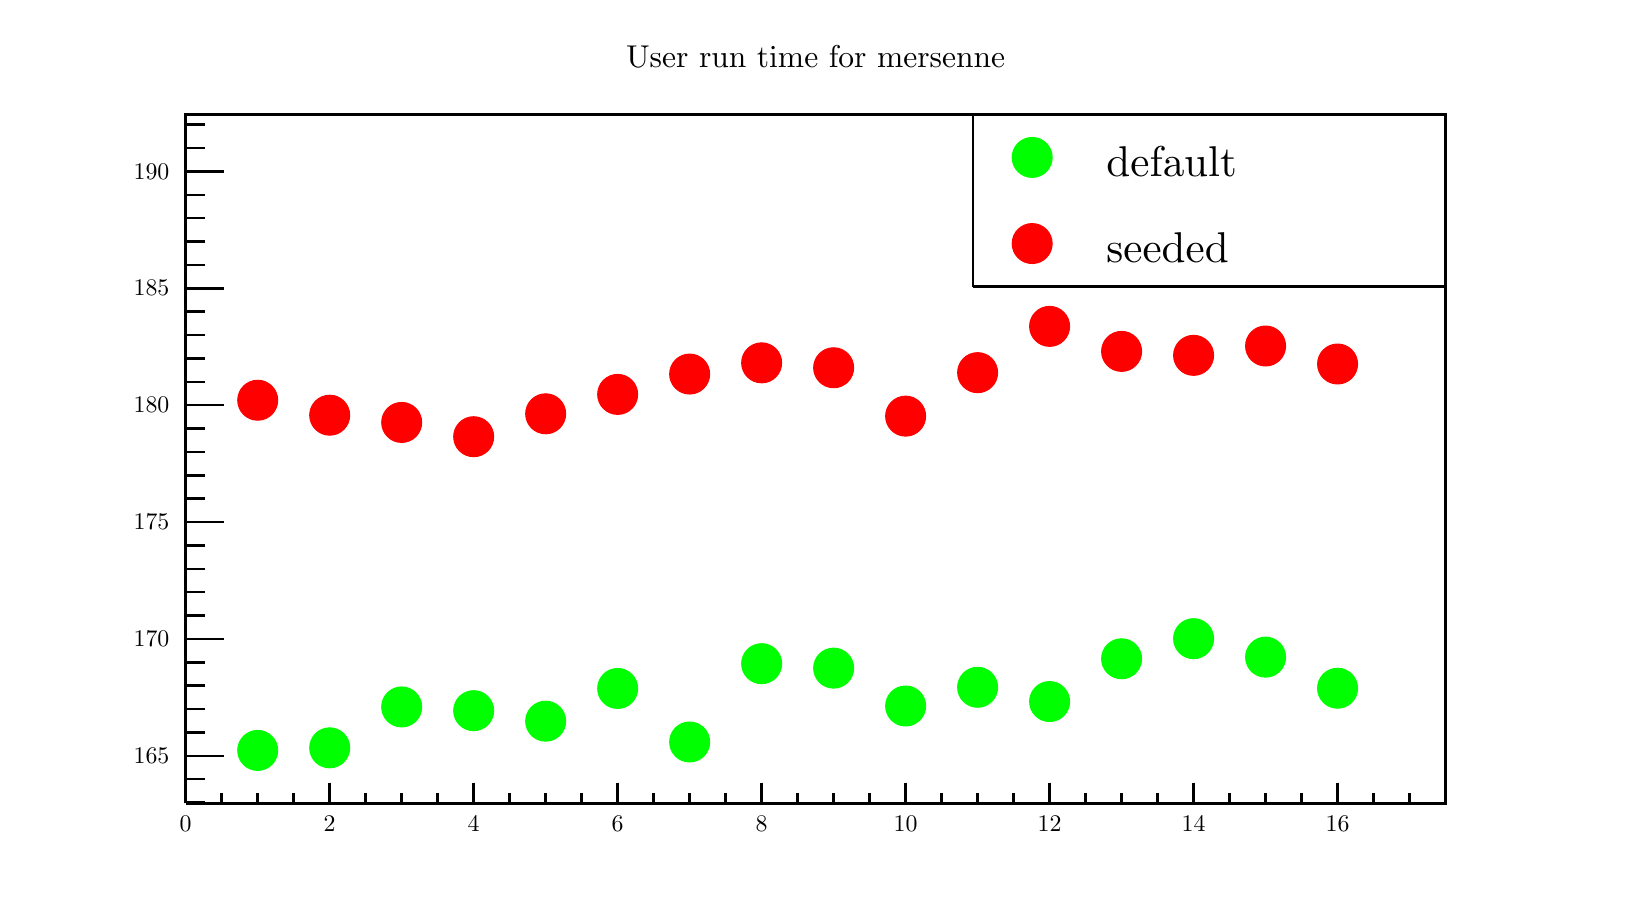
\begin{tikzpicture}
\pgfdeclareplotmark{cross} {
\pgfpathmoveto{\pgfpoint{-0.3\pgfplotmarksize}{\pgfplotmarksize}}
\pgfpathlineto{\pgfpoint{+0.3\pgfplotmarksize}{\pgfplotmarksize}}
\pgfpathlineto{\pgfpoint{+0.3\pgfplotmarksize}{0.3\pgfplotmarksize}}
\pgfpathlineto{\pgfpoint{+1\pgfplotmarksize}{0.3\pgfplotmarksize}}
\pgfpathlineto{\pgfpoint{+1\pgfplotmarksize}{-0.3\pgfplotmarksize}}
\pgfpathlineto{\pgfpoint{+0.3\pgfplotmarksize}{-0.3\pgfplotmarksize}}
\pgfpathlineto{\pgfpoint{+0.3\pgfplotmarksize}{-1.\pgfplotmarksize}}
\pgfpathlineto{\pgfpoint{-0.3\pgfplotmarksize}{-1.\pgfplotmarksize}}
\pgfpathlineto{\pgfpoint{-0.3\pgfplotmarksize}{-0.3\pgfplotmarksize}}
\pgfpathlineto{\pgfpoint{-1.\pgfplotmarksize}{-0.3\pgfplotmarksize}}
\pgfpathlineto{\pgfpoint{-1.\pgfplotmarksize}{0.3\pgfplotmarksize}}
\pgfpathlineto{\pgfpoint{-0.3\pgfplotmarksize}{0.3\pgfplotmarksize}}
\pgfpathclose
\pgfusepathqstroke
}
\pgfdeclareplotmark{cross*} {
\pgfpathmoveto{\pgfpoint{-0.3\pgfplotmarksize}{\pgfplotmarksize}}
\pgfpathlineto{\pgfpoint{+0.3\pgfplotmarksize}{\pgfplotmarksize}}
\pgfpathlineto{\pgfpoint{+0.3\pgfplotmarksize}{0.3\pgfplotmarksize}}
\pgfpathlineto{\pgfpoint{+1\pgfplotmarksize}{0.3\pgfplotmarksize}}
\pgfpathlineto{\pgfpoint{+1\pgfplotmarksize}{-0.3\pgfplotmarksize}}
\pgfpathlineto{\pgfpoint{+0.3\pgfplotmarksize}{-0.3\pgfplotmarksize}}
\pgfpathlineto{\pgfpoint{+0.3\pgfplotmarksize}{-1.\pgfplotmarksize}}
\pgfpathlineto{\pgfpoint{-0.3\pgfplotmarksize}{-1.\pgfplotmarksize}}
\pgfpathlineto{\pgfpoint{-0.3\pgfplotmarksize}{-0.3\pgfplotmarksize}}
\pgfpathlineto{\pgfpoint{-1.\pgfplotmarksize}{-0.3\pgfplotmarksize}}
\pgfpathlineto{\pgfpoint{-1.\pgfplotmarksize}{0.3\pgfplotmarksize}}
\pgfpathlineto{\pgfpoint{-0.3\pgfplotmarksize}{0.3\pgfplotmarksize}}
\pgfpathclose
\pgfusepathqfillstroke
}
\pgfdeclareplotmark{newstar} {
\pgfpathmoveto{\pgfqpoint{0pt}{\pgfplotmarksize}}
\pgfpathlineto{\pgfqpointpolar{44}{0.5\pgfplotmarksize}}
\pgfpathlineto{\pgfqpointpolar{18}{\pgfplotmarksize}}
\pgfpathlineto{\pgfqpointpolar{-20}{0.5\pgfplotmarksize}}
\pgfpathlineto{\pgfqpointpolar{-54}{\pgfplotmarksize}}
\pgfpathlineto{\pgfqpointpolar{-90}{0.5\pgfplotmarksize}}
\pgfpathlineto{\pgfqpointpolar{234}{\pgfplotmarksize}}
\pgfpathlineto{\pgfqpointpolar{198}{0.5\pgfplotmarksize}}
\pgfpathlineto{\pgfqpointpolar{162}{\pgfplotmarksize}}
\pgfpathlineto{\pgfqpointpolar{134}{0.5\pgfplotmarksize}}
\pgfpathclose
\pgfusepathqstroke
}
\pgfdeclareplotmark{newstar*} {
\pgfpathmoveto{\pgfqpoint{0pt}{\pgfplotmarksize}}
\pgfpathlineto{\pgfqpointpolar{44}{0.5\pgfplotmarksize}}
\pgfpathlineto{\pgfqpointpolar{18}{\pgfplotmarksize}}
\pgfpathlineto{\pgfqpointpolar{-20}{0.5\pgfplotmarksize}}
\pgfpathlineto{\pgfqpointpolar{-54}{\pgfplotmarksize}}
\pgfpathlineto{\pgfqpointpolar{-90}{0.5\pgfplotmarksize}}
\pgfpathlineto{\pgfqpointpolar{234}{\pgfplotmarksize}}
\pgfpathlineto{\pgfqpointpolar{198}{0.5\pgfplotmarksize}}
\pgfpathlineto{\pgfqpointpolar{162}{\pgfplotmarksize}}
\pgfpathlineto{\pgfqpointpolar{134}{0.5\pgfplotmarksize}}
\pgfpathclose
\pgfusepathqfillstroke
}
\definecolor{c}{rgb}{1,1,1};
\draw [color=c, fill=c] (0,0) rectangle (20,10.9387);
\draw [color=c, fill=c] (2,1.09387) rectangle (18,9.84481);
\definecolor{c}{rgb}{0,0,0};
\draw [c,line width=0.9] (2,1.09387) -- (2,9.84481) -- (18,9.84481) -- (18,1.09387) -- (2,1.09387);
\definecolor{c}{rgb}{1,1,1};
\draw [color=c, fill=c] (2,1.09387) rectangle (18,9.84481);
\definecolor{c}{rgb}{0,0,0};
\draw [c,line width=0.9] (2,1.09387) -- (2,9.84481) -- (18,9.84481) -- (18,1.09387) -- (2,1.09387);
\draw [c,line width=0.9] (2,1.09387) -- (18,1.09387);
\draw [c,line width=0.9] (2,1.3564) -- (2,1.09387);
\draw [c,line width=0.9] (2.45714,1.22513) -- (2.45714,1.09387);
\draw [c,line width=0.9] (2.91429,1.22513) -- (2.91429,1.09387);
\draw [c,line width=0.9] (3.37143,1.22513) -- (3.37143,1.09387);
\draw [c,line width=0.9] (3.82857,1.3564) -- (3.82857,1.09387);
\draw [c,line width=0.9] (4.28571,1.22513) -- (4.28571,1.09387);
\draw [c,line width=0.9] (4.74286,1.22513) -- (4.74286,1.09387);
\draw [c,line width=0.9] (5.2,1.22513) -- (5.2,1.09387);
\draw [c,line width=0.9] (5.65714,1.3564) -- (5.65714,1.09387);
\draw [c,line width=0.9] (6.11429,1.22513) -- (6.11429,1.09387);
\draw [c,line width=0.9] (6.57143,1.22513) -- (6.57143,1.09387);
\draw [c,line width=0.9] (7.02857,1.22513) -- (7.02857,1.09387);
\draw [c,line width=0.9] (7.48571,1.3564) -- (7.48571,1.09387);
\draw [c,line width=0.9] (7.94286,1.22513) -- (7.94286,1.09387);
\draw [c,line width=0.9] (8.4,1.22513) -- (8.4,1.09387);
\draw [c,line width=0.9] (8.85714,1.22513) -- (8.85714,1.09387);
\draw [c,line width=0.9] (9.31429,1.3564) -- (9.31429,1.09387);
\draw [c,line width=0.9] (9.77143,1.22513) -- (9.77143,1.09387);
\draw [c,line width=0.9] (10.2286,1.22513) -- (10.2286,1.09387);
\draw [c,line width=0.9] (10.6857,1.22513) -- (10.6857,1.09387);
\draw [c,line width=0.9] (11.1429,1.3564) -- (11.1429,1.09387);
\draw [c,line width=0.9] (11.6,1.22513) -- (11.6,1.09387);
\draw [c,line width=0.9] (12.0571,1.22513) -- (12.0571,1.09387);
\draw [c,line width=0.9] (12.5143,1.22513) -- (12.5143,1.09387);
\draw [c,line width=0.9] (12.9714,1.3564) -- (12.9714,1.09387);
\draw [c,line width=0.9] (13.4286,1.22513) -- (13.4286,1.09387);
\draw [c,line width=0.9] (13.8857,1.22513) -- (13.8857,1.09387);
\draw [c,line width=0.9] (14.3429,1.22513) -- (14.3429,1.09387);
\draw [c,line width=0.9] (14.8,1.3564) -- (14.8,1.09387);
\draw [c,line width=0.9] (15.2571,1.22513) -- (15.2571,1.09387);
\draw [c,line width=0.9] (15.7143,1.22513) -- (15.7143,1.09387);
\draw [c,line width=0.9] (16.1714,1.22513) -- (16.1714,1.09387);
\draw [c,line width=0.9] (16.6286,1.3564) -- (16.6286,1.09387);
\draw [c,line width=0.9] (16.6286,1.3564) -- (16.6286,1.09387);
\draw [c,line width=0.9] (17.0857,1.22513) -- (17.0857,1.09387);
\draw [c,line width=0.9] (17.5429,1.22513) -- (17.5429,1.09387);
\draw [c,line width=0.9] (18,1.22513) -- (18,1.09387);
\draw [anchor=base] (2,0.732891) node[scale=0.861703, color=c, rotate=0]{0};
\draw [anchor=base] (3.82857,0.732891) node[scale=0.861703, color=c, rotate=0]{2};
\draw [anchor=base] (5.65714,0.732891) node[scale=0.861703, color=c, rotate=0]{4};
\draw [anchor=base] (7.48571,0.732891) node[scale=0.861703, color=c, rotate=0]{6};
\draw [anchor=base] (9.31429,0.732891) node[scale=0.861703, color=c, rotate=0]{8};
\draw [anchor=base] (11.1429,0.732891) node[scale=0.861703, color=c, rotate=0]{10};
\draw [anchor=base] (12.9714,0.732891) node[scale=0.861703, color=c, rotate=0]{12};
\draw [anchor=base] (14.8,0.732891) node[scale=0.861703, color=c, rotate=0]{14};
\draw [anchor=base] (16.6286,0.732891) node[scale=0.861703, color=c, rotate=0]{16};
\draw [c,line width=0.9] (2,1.09387) -- (2,9.84481);
\draw [c,line width=0.9] (2.48,1.69874) -- (2,1.69874);
\draw [c,line width=0.9] (2.24,1.99561) -- (2,1.99561);
\draw [c,line width=0.9] (2.24,2.29247) -- (2,2.29247);
\draw [c,line width=0.9] (2.24,2.58934) -- (2,2.58934);
\draw [c,line width=0.9] (2.24,2.88621) -- (2,2.88621);
\draw [c,line width=0.9] (2.48,3.18308) -- (2,3.18308);
\draw [c,line width=0.9] (2.24,3.47995) -- (2,3.47995);
\draw [c,line width=0.9] (2.24,3.77682) -- (2,3.77682);
\draw [c,line width=0.9] (2.24,4.07368) -- (2,4.07368);
\draw [c,line width=0.9] (2.24,4.37055) -- (2,4.37055);
\draw [c,line width=0.9] (2.48,4.66742) -- (2,4.66742);
\draw [c,line width=0.9] (2.24,4.96429) -- (2,4.96429);
\draw [c,line width=0.9] (2.24,5.26116) -- (2,5.26116);
\draw [c,line width=0.9] (2.24,5.55803) -- (2,5.55803);
\draw [c,line width=0.9] (2.24,5.85489) -- (2,5.85489);
\draw [c,line width=0.9] (2.48,6.15176) -- (2,6.15176);
\draw [c,line width=0.9] (2.24,6.44863) -- (2,6.44863);
\draw [c,line width=0.9] (2.24,6.7455) -- (2,6.7455);
\draw [c,line width=0.9] (2.24,7.04237) -- (2,7.04237);
\draw [c,line width=0.9] (2.24,7.33924) -- (2,7.33924);
\draw [c,line width=0.9] (2.48,7.6361) -- (2,7.6361);
\draw [c,line width=0.9] (2.24,7.93297) -- (2,7.93297);
\draw [c,line width=0.9] (2.24,8.22984) -- (2,8.22984);
\draw [c,line width=0.9] (2.24,8.52671) -- (2,8.52671);
\draw [c,line width=0.9] (2.24,8.82358) -- (2,8.82358);
\draw [c,line width=0.9] (2.48,9.12045) -- (2,9.12045);
\draw [c,line width=0.9] (2.48,1.69874) -- (2,1.69874);
\draw [c,line width=0.9] (2.24,1.40187) -- (2,1.40187);
\draw [c,line width=0.9] (2.24,1.105) -- (2,1.105);
\draw [c,line width=0.9] (2.48,9.12045) -- (2,9.12045);
\draw [c,line width=0.9] (2.24,9.41732) -- (2,9.41732);
\draw [c,line width=0.9] (2.24,9.71418) -- (2,9.71418);
\draw [anchor= east] (1.9,1.69874) node[scale=0.861703, color=c, rotate=0]{165};
\draw [anchor= east] (1.9,3.18308) node[scale=0.861703, color=c, rotate=0]{170};
\draw [anchor= east] (1.9,4.66742) node[scale=0.861703, color=c, rotate=0]{175};
\draw [anchor= east] (1.9,6.15176) node[scale=0.861703, color=c, rotate=0]{180};
\draw [anchor= east] (1.9,7.6361) node[scale=0.861703, color=c, rotate=0]{185};
\draw [anchor= east] (1.9,9.12045) node[scale=0.861703, color=c, rotate=0]{190};
\definecolor{c}{rgb}{0,1,0};
\foreach \P in {(2.91429,1.76702), (3.82857,1.79967), (4.74286,2.31919), (5.65714,2.27169), (6.57143,2.1381), (7.48571,2.55372), (8.4,1.87389), (9.31429,2.8684), (10.2286,2.81199), (11.1429,2.33107), (12.0571,2.56856), (12.9714,2.38747),
 (13.8857,2.93074), (14.8,3.18605), (15.7143,2.95152), (16.6286,2.55669)}{\draw[mark options={color=c,fill=c},mark size=7.207207pt,mark=*] plot coordinates {\P};}
\definecolor{c}{rgb}{1,0,0};
\foreach \P in {(2.91429,6.21411), (3.82857,6.02411), (4.74286,5.93208), (5.65714,5.75099), (6.57143,6.04192), (7.48571,6.28832), (8.4,6.5466), (9.31429,6.68909), (10.2286,6.62675), (11.1429,6.01223), (12.0571,6.56441), (12.9714,7.15221),
 (13.8857,6.83456), (14.8,6.78409), (15.7143,6.90284), (16.6286,6.67425)}{\draw[mark options={color=c,fill=c},mark size=7.207207pt,mark=*] plot coordinates {\P};}
\definecolor{c}{rgb}{1,1,1};
\draw [color=c, fill=c] (12,7.65707) rectangle (18,9.84481);
\definecolor{c}{rgb}{0,0,0};
\draw [c,line width=0.9] (12,7.65707) -- (18,7.65707);
\draw [c,line width=0.9] (18,7.65707) -- (18,9.84481);
\draw [c,line width=0.9] (18,9.84481) -- (12,9.84481);
\draw [c,line width=0.9] (12,9.84481) -- (12,7.65707);
\draw [anchor=base west] (13.5,9.05175) node[scale=1.55662, color=c, rotate=0]{default};
\definecolor{c}{rgb}{1,1,1};
\draw [c] (12.225,8.91502) -- (13.275,8.91502) -- (13.275,9.68073) -- (12.225,9.68073);
\draw [c,line width=0.9] (12.225,9.29787) -- (13.275,9.29787);
\definecolor{c}{rgb}{0,1,0};
\foreach \P in {(12.75,9.29787)}{\draw[mark options={color=c,fill=c},mark size=7.207207pt,mark=*] plot coordinates {\P};}
\definecolor{c}{rgb}{0,0,0};
\draw [anchor=base west] (13.5,7.95788) node[scale=1.55662, color=c, rotate=0]{seeded};
\definecolor{c}{rgb}{1,1,1};
\draw [c] (12.225,7.82115) -- (13.275,7.82115) -- (13.275,8.58686) -- (12.225,8.58686);
\draw [c,line width=0.9] (12.225,8.20401) -- (13.275,8.20401);
\definecolor{c}{rgb}{1,0,0};
\foreach \P in {(12.75,8.20401)}{\draw[mark options={color=c,fill=c},mark size=7.207207pt,mark=*] plot coordinates {\P};}
\definecolor{c}{rgb}{0,0,0};
\draw (10,10.5832) node[scale=1.13967, color=c, rotate=0]{User run time for mersenne};
\end{tikzpicture}
